% \documentclass[12pt,handout,xcolor=pdftex,dvipsnames,table]{beamer} %For handouts.
\documentclass[xcolor=pdftex,dvipsnames,table]{beamer}
%\usepackage{pgfpages} %For handouts.
% This is the file main.tex
% \usepackage{handoutWithNotes}
\usepackage{graphicx}
\usepackage[en-US]{datetime2} % fix warning of \author[*]{\today}
\usepackage{lmodern}% http://ctan.org/pkg/lm (For special Fonts)
\usepackage{ragged2e} % justify document

\mode<presentation>
\setbeamertemplate{blocks}[rounded][shadow=true]
\usetheme{Dresden} % so so
\setbeamertemplate{navigation symbols}{} %take out the navigation symbols
\setbeamertemplate{caption}[numbered] %enumerate the caption and tables
\usefonttheme[stillsansseriflarge]{structureitalicserif}
\expandafter\def\expandafter\insertshorttitle\expandafter{%
  \insertshorttitle\hfill\insertframenumber\,/\,\inserttotalframenumber}%page numbering
  
%\mode<handout>{\setbeamercolor{background canvas}{bg=black!5}} %For handouts.
% \pgfpagesuselayout{4 on 1 with notes}[a4paper,border shrink=5mm]
  
%\makeatletter %reset the numbering on the subfigures (1)
%\@addtoreset{subfigure}{figure} %reset the numbering on the subfigures (2)
%\makeatother %reset the numbering on the subfigures (3)

%For Large figures
%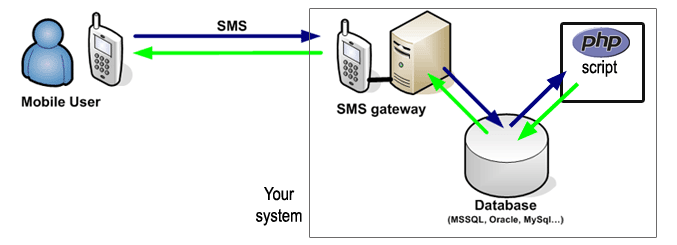
\includegraphics[width=\linewidth,height=\textheight,keepaspectratio]{SMS}

\title{Demonstration User Manual} % (optional, only for long titles)
\subtitle{
  \href{https://github.com/thanos1983/Python2-Dango-REST-API}
    {GitHub Project: Python2-Dango-REST-API} }
\author[Athanasios Garyfalos]{Last Update: \today} % (optional, for multiple authors)
% {A.~Garyfalos \and A.~Garyfalos2 \and A.~Garyfalos3}
\institute[garyfalos@cpan.org] % (optional)
{
\\
\medskip
{
% \emph{A.atga12@student.bth.se}
% \emph{Another Author email}
% \emph{Another Author}
}
}
% \vspace*{-11.5em}
% \date{Date: \today}
% \subject{Sample of Work Demonstration Django Rest Framework}

\begin{document}

\begin{frame}[noframenumbering]
  \begin{center}
    % Upper part of the page
    % \vspace*{5.0em}
    
\includegraphics[width=.8\textwidth]{png/djangoRestLogo}\\ [0.3cm]    

    % \emph{Supervisor:} \\  
    % Prof.~Kulesza\\
    % \textsc{Wlodek} 
  \end{center}
  \titlepage
\end{frame}

\section*{Copyright Disclaimer}
  \begin{frame}
    \begin{justify}
      {\justifying Copyright \alert{Disclaimer}: This program is free software: you can redistribute it and/or modify it under the terms of the GNU General Public License as published by the Free Software Foundation, either version 3 of the License, or (at your option) any later version.
      \bigbreak
      This program is distributed in the hope that it will be useful, but WITHOUT ANY WARRANTY; without even the implied warranty of MERCHANTABILITY or FITNESS FOR A PARTICULAR PURPOSE.  See the GNU General Public License for more details.
      \bigbreak
      You should have received a copy of the GNU General Public License along with this program.  If not, see.~\cite{gnuLicences} }
    \end{justify}
\end{frame}

\section*{Contents}
\begin{frame}
\setbeamercovered{dynamic}%Makes the text appear before it presents nice!!!! 
\frametitle{Outline}
\tableofcontents[pausesections]
\end{frame}

\section{Group Members}
\label{sec:group}

\subsection{Group members positions and responsibilities}
  
\begin{frame}
\setbeamercovered{dynamic}%Makes the text appear before it presents nice!!!! 
  \begin{exampleblock}{SNMP group members}
    \begin{itemize}
      \item Positions
      \item<1-| alert@1>> Athanasios Garyfalos (\alert{Project Manager})
      \item<2-| alert@2>> Taha Mohammad (\alert{Research and Development RnD})
      \item<3-| alert@3>> Jaroslaw Rykaczewski (\alert{Software Engineering})
      \item Responsibilities
      \item<1-| alert@1>> Planning-executing-closing the project based on deadlines.
      \item<2-| alert@2>> Develop new ideas and products. Will give us the competitive edge.
      \item<3-| alert@3>> Develop and implement the ideas of the RnD.
    \end{itemize}
  \end{exampleblock}
\end{frame}

% \section{Wireless Platform}
\label{sec:wireless}
  \subsection{Key Factors and Components}

\begin{frame}{Hardware Description}
\setbeamercovered{dynamic}%Makes the text appear before it presents nice!!!!
    \begin{columns}[t] % contents are top vertically aligned
      \begin{column}[T]{5cm} % each column can also be its own environment
        \begin{itemize}
            \item<+-| alert@+> Single component of the base winding Figure:%~\autoref{fig:structure}.
            \item<+-| alert@+> Receiver platform values Figure:~1b.
            \item<+-| alert@+> Worst coupling position Figure:~1c.
            \item<+-| alert@+> Best coupling position Figure:~1d.
          \end{itemize}  
      \end{column}
    \begin{column}[T]{5cm} % alternative top-align that's better for graphics
      \begin{figure}
        \only<1>{%
        %\vspace*{-1.5cm}
          \subfloat[First subfigure\label{fig:a}]{
            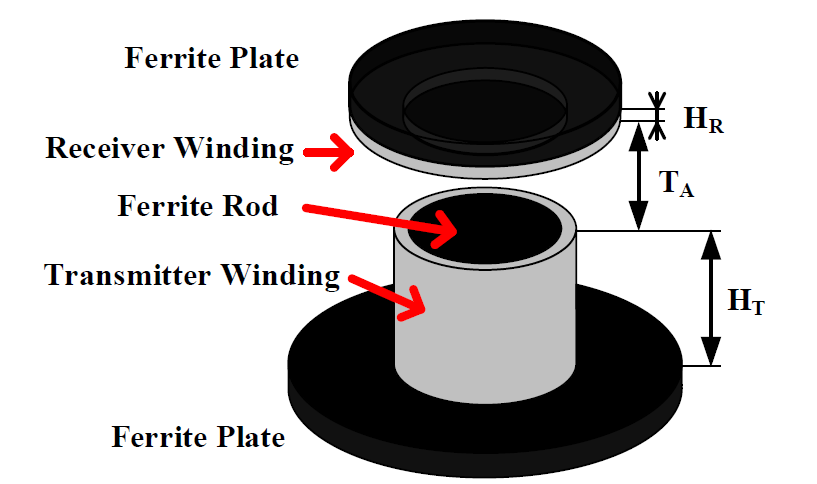
\includegraphics[height=2cm,width=3cm]{./png/structure}
          }
          \label{fig:1}
        }
        \only<2>{%
        %\vspace*{-1.5cm}
          \subfloat[Second subfigure\label{fig:b}]{
            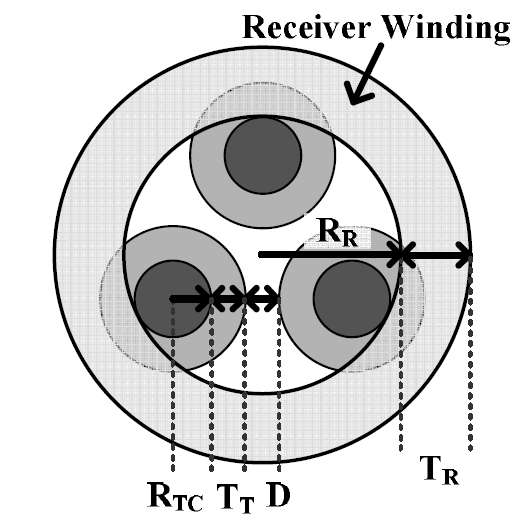
\includegraphics[height=2cm,width=3cm]{./png/receiver}
          }
          \label{fig:2}
        }
        \only<3>{%
        %\vspace*{-1.5cm}
          \subfloat[Third subfigure\label{fig:c}]{
            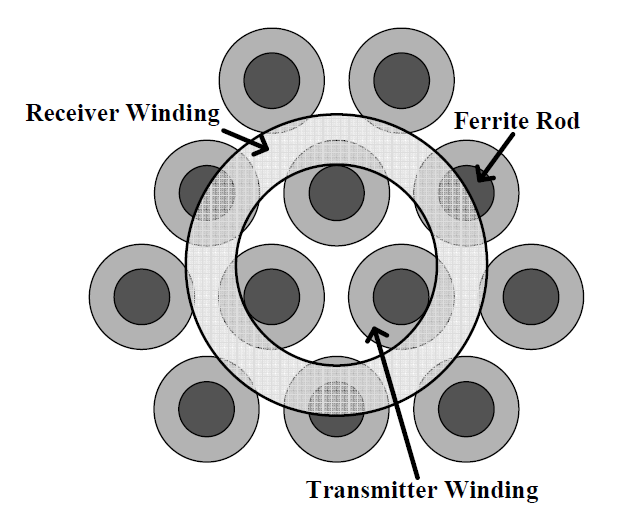
\includegraphics[height=2cm,width=3cm]{./png/worst}
          }
          \label{fig:3}
        }
        \only<4>{%
        %\vspace*{-1.5cm}
          \subfloat[Fourth subfigure\label{fig:d}]{
            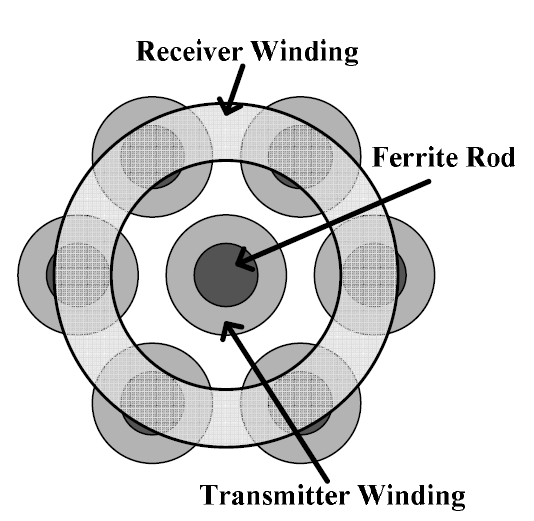
\includegraphics[height=2cm,width=3cm]{./png/best}
          }
          \label{fig:4}
        }
        \captionsetup{justification=centering} %Center a two line caption
        \caption{Project Positioning Analysis} \protect\label{fig:5}%~\cite{wsn}
      \end{figure}
    \end{column}
  \end{columns}
\end{frame}

%\subsection{Best and Worst Performance Based on Positioning}

%\begin{frame}{Theory Vs Practical Experimentation}
%\setbeamercovered{dynamic}%Makes the text appear before it presents nice!!!! 
%    \begin{columns}[t] % contents are top vertically aligned
%      \begin{column}[T]{5cm} % each column can also be its own environment
%        \begin{itemize}
%            \item<+-| alert@+> Best Position Simulation (\ding{108})
%            \item<+-| alert@+> Worst Position Simulation (\alert{\ding{110}})
%            \item<+-| alert@+> Best Position Measured (\ding{108})
%            \item<+-| alert@+> Worst Position Measured (\alert{\ding{110}})
%            \item<+-| alert@+> Simulation is a perfect line, in ``\alert{Theory}''
%            \item<+-| alert@+> Practical measuring shows ``\alert{150KHz}''!
%        \end{itemize}
%      \end{column}
%    \begin{column}[T]{5cm} % alternative top-align that's better for graphics
%      \begin{figure}
%        \vspace*{-10pt}
%        \centerline{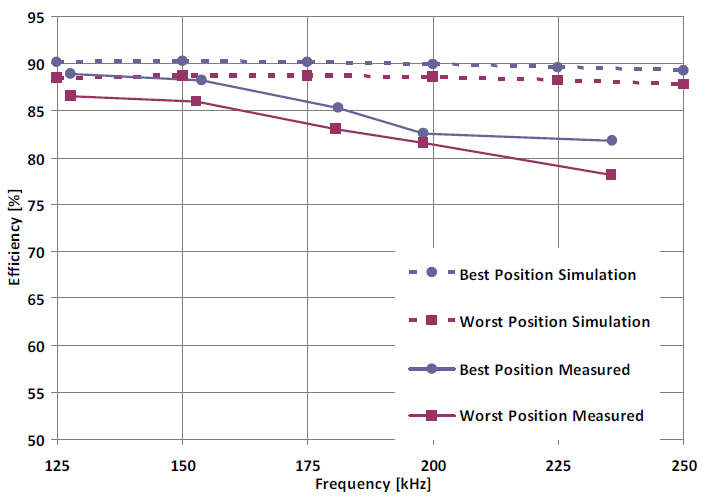
\includegraphics[scale=0.7]{./png/efficiency}}
%        \vspace*{10pt}
%        \captionsetup{justification=centering} %Center a two line caption
%        \caption{Simulation Vs Real Time Efficiency~\cite{wsn}}
        %\includegraphics[options]{path_to_image}syntax
%      \end{figure}
%    \end{column}
%  \end{columns}
%\end{frame}

% \section{Implementation}
\label{sec:implementation}
  \subsection{Neural Network Algorithm Implementation}
  
\begin{frame}
  \centering
  \begin{figure}
    \only<1-3>{
        \begin{subfigure}[b]{0.3\textwidth}
          \caption{Free Positioning}
                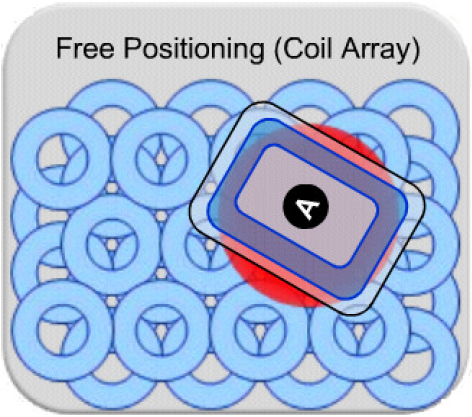
\includegraphics[width=\textwidth,height=\textwidth]{./png/multiple}
                \label{fig:guided}
                \setcounter{subfigure}{0}% Reset subfigure counter
        \end{subfigure}\hfill
        }
    \only<2-3>{
        ~ %add desired spacing between images, e. g. ~, \quad, \qquad etc.
          %(or a blank line to force the subfigure onto a new line)
        \begin{subfigure}[b]{0.3\textwidth}
        \setcounter{subfigure}{1}% Reset subfigure counter
          \caption{Neural Network}
                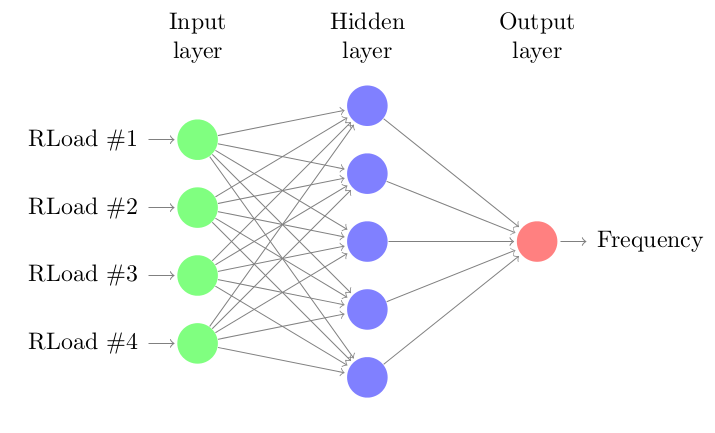
\includegraphics[width=\textwidth,height=\textwidth]{./png/neural}
                \label{fig:free}
        \setcounter{subfigure}{0}% Reset subfigure counter
        \end{subfigure}\hfill
        }
    \only<3-3>{
        ~ %add desired spacing between images, e. g. ~, \quad, \qquad etc.
          %(or a blank line to force the subfigure onto a new line)
        \begin{subfigure}[b]{0.3\textwidth}
            \setcounter{subfigure}{2}% Reset subfigure counter
          \caption{Matlab Output}
                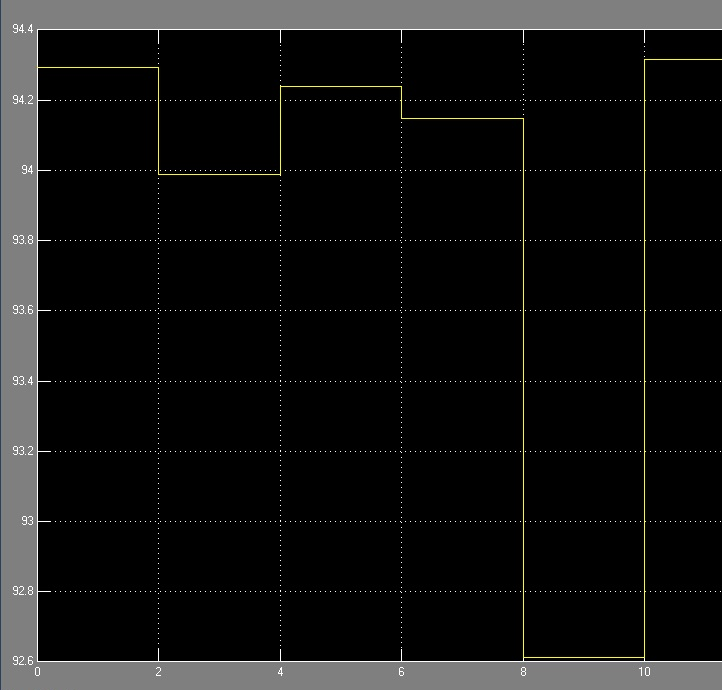
\includegraphics[width=\textwidth,height=\textwidth]{./png/output}
                \label{fig:multiple}
        \end{subfigure}%
        }
        \caption{Different wireless charging approaches~\label{fig:animals}~\cite{wsn}}
  \end{figure}
  \begin{itemize}[<+->]
      \item<1-| alert@1>> Free positioning charging based on Inductive coupling~\cite{wireless}.
      \item<2-| alert@2>> Based on RLoad and Frequency Input and Output ~\cite{wireless}. %\ref{fig:free}
      \item<3-| alert@3>> Simulation of Matlab Output based on RLoad as an Input~\cite{wireless}. %\ref{fig:multiple}
    \end{itemize} 
\end{frame}

% \section{Summary}
  \subsection{Key points repetition}

\begin{frame}
\setbeamercovered{dynamic}
  \begin{exampleblock}{Summary}
    \begin{itemize}[<+->]
      \item In section~``\nameref{sec:group}'' page ``\ref{sec:group}'' we mentioned member positions and responsibilities. 
      \item In section~``\nameref{sec:wireless}'' page ``\ref{sec:wireless}'' we mentioned hardware components and best/worst positions.
      \item In section~``\nameref{sec:implementation}'' page ``\ref{sec:implementation}'' we mentioned our approach and proposed solution to the problem \pause
    \end{itemize}
  \end{exampleblock}
  \begin{exampleblock}{Extra Notes}
    \begin{itemize}[<+->]
      \item Both the Conference paper and the Presentation where written in \alert{\LaTeX}
      \item Due to the quality of the output it exceeds our expectations!~\cite{research}
    \end{itemize}
  \end{exampleblock}
\end{frame}

\subsection*{Questions}
\begin{frame}
%\begin{overlayarea}{\textwidth}{3cm}
    %\only<1>{Some text for the first slide.\\Possibly several lines long.}
    %\only<2>{Replacement on the second slide.}
%\end{overlayarea}
  \begin{itemize}
     \Large
    \item \colorbox{yellow}{Thanks a lot – questions \& comments?}
  \end{itemize} 
\end{frame}

\section{Bibliography}
\subsection*{Web and Articles}

\begin{frame}[allowframebreaks]
  \frametitle<presentation>{References}
  \bibliographystyle{amsalpha}   
  \begin{thebibliography}{10}
    %\setbeamertemplate{bibliography item}[online]
    \setbeamertemplate{bibliography item}{
\includegraphics[width=1.5em]{./png/gnu}}
    \bibitem{gnuLicences}
      GNU LESSER GENERAL PUBLIC LICENSE
      \newblock {\emph{GNU Operating System}}
      \newblock available at \url{https://www.gnu.org/licenses/lgpl.html}.
    %\setbeamertemplate{bibliography item}[online]
    \setbeamertemplate{bibliography item}{
\includegraphics[width=1.5em]{./png/www}}
    \bibitem{djangoRestFramework}
      Author: T.~Christie
      \newblock {\emph{Django Rest Framework Project}}
      \newblock available at \url{http://www.django-rest-framework.org}.
    \setbeamertemplate{bibliography item}[article]
    \setbeamertemplate{bibliography item}{
\includegraphics[width=1.3em]{./png/heroku}}
    \bibitem{herokuApi}
      Author: A.~Garyfalos
      \newblock {\emph{thanos-test.herokuapp}}
      \newblock available at \url{https://thanos-test.herokuapp.com}.
  \end{thebibliography}
\end{frame}

\end{document}
